\documentclass{Assignment}
\usepackage{tikz}
\usepackage{pdfpages}
\usetikzlibrary{graphs}
\title{Graph Theory}
\begin{document}

\section*{Task 1}
\subsection*{Introduction}
Main idea of this project is to understand graphs  as a mathematical set and also in a computer science perspective. Generally graphs are thought of as usually thought of as functions that are made of axis i.e x and y, and well the z-th axis. But mathematicians usually study graphs made up of set of vertices(points) with edges(curves) connecting these vertices. And these graphs have various applications in our real lives, this includes flight paths, social networks like friend groups and puzzle games. In this project our main focus would be on complete graphs.\\
\\
 I started preparing researching by starting with firstly this stage, understanding what a simple graph is, from a mathematical view point and how it can be understood from a computer science view point. From graphs we get to the Ramsey theory which is a problem relating to graphs theory and very hard to solve. Ramsey theory tries to understand how order is found in chaos. And from my understanding is Ramsey numbers are hard to find because the graphs that are generated depending on the vertices grow super-exponentially by a factor of $2^{n^2}$ this is the reason why Ramsey numbers of diagonals over 4 are not yet found.\\
  
\section*{Sub task A}
\subsection*{Graph Theory}
Graph- A graph $G = (V,E)$ is a set of objects called vertices $V$ and a pair of objects taken from $V$ called edges.\\
$V = \{v_1,v_2,v_3....\}$\\
$E = \{e_{12},e_{13}...\}$\\\\
Neighbours- Two vertices that are connected by an edge\\\\
Degree - Number of edges connected to a vertex\\\\
Directed Graph - edges have orientation\\\\
Undirected Graph -  edges have no orientation\\\\
Complete Graph $K_n$
\begin{itemize}
	\item has n vertices and all possible edges 
	\item has degrees n-1
	\item number of edges is $\frac{n(n-1)}{2}$
\end{itemize}
Adjacent Matrix\\
$$\begin{tikzpicture}
	\graph {
		1 -- {2};
		2--{3};
		3--{1};
		4--{3};

	};
\end{tikzpicture}$$
$$\begin{tabular}{c|c|c|c|c}
		&1&2&3&4\\\hline
		1&0&1&1&0\\\hline
		2&1&0&1&0\\\hline
		3&1&1&0&1\\\hline
		4&0&0&1&0\\\hline
\end{tabular}$$'
Adjacent List \\\\
\begin{center}
1 $\rightarrow$(2,3)\\
2 $\rightarrow$(1,3)\\
3 $\rightarrow$(1,2,4)\\
4 $\rightarrow$(3)\end{center}
\underline{Several applications of Graphs}\\\\
\begin{itemize}
	\item Mappings/Navigation (Uber)
	\item Social Network
	\item Puzzle games (Soduku, Chess)
\end{itemize}
\newpage
\subsection*{Ramsey Theory}
Named after mathematician Frank Ramsey, who first proved a problem in combinatorics.\\
The theory state that a monochromatic cliques in any edge labeling of large enough complete graph, or for two colours say red(r) and blue(b) be any two positive integers, the theorem states that there's a least positive integer $R(r,b)$ such that for which every blue-red edge colouring of the complete graph on $R(r,b)$ vertices contains a blue clique on r vertices or a red clique on b vertices.\\\\
\begin{itemize}
	\item In a complex and large enough system a pattern can almost be found
	\item There is order in chaos
	\item Made up of complete graphs
\end{itemize}
\subsection*{Ramsey Numbers}
Is the minimum number of vertices $n = R(r,b)$ such that all undirected simple graph of order r contains a group of order b or independent set of order n
\newpage
\section*{Sub Task B}
\begin{enumerate}
	\item n Represents the minimum number such that the complete graph $k_n$ gives for every blue-red colouring of $k_n$ a blue-coloured $k_l$ or a red-coloured $k_t$.\\\\
	When k/l or k and l are increased, we get a bigger n, this shows that n depends on k and l\\\\
	Example(The party problem)\\\\
	How many people(n) are needed to be invited to a party to guarantee that either k people know each other or l people are strangers 
	\item 
	Starting from the known Ramsey Numbers, k and l = 1, only considering the diagonal ones where k=l\\\\
	R(1,1)=1\\
	R(2,2)=2\\
	R(3,3) = 6\\
	R(4,4)=18\\
Showing that the n increases with an increase in both k and l
\end{enumerate}
\subsection*{Summary}
Firstly what i did was use the links provided to understand the theories given namely Graph Theory and Ramsey Theory. Understanding concept of graphs from a mathematical point of view together with computer science point of view. We explored applications in different fields and how they are incredibly not easy to compute. And understood that there exists order in chaos.
\newpage
\section*{Task 2}

\subsection*{Introduction}
Main idea is that graphs can have different orientations but same structure this is called homomorphic graphs. So what i understand in this task is to see how we can get different structures of graphs from making orientations with the vertices and edges. Each vertices in different graphs say graph A and graph B must first have same about of vertices that can be arranged in any orientation, same degrees and with same number of neighbours in other words this can be thought of as same graphs that have same structural properties. Its more about fitting one graph into the other by shifting vertices and edges but still preserving the same structure. \\\\
So for this task I was able to draw different graphs starting with graph of only one vertices having no edges to going to in increasing manner from 2, 3 and 4 vertices. What happened is i explored different types of orientations and how the number of graphs depends on the number $2^{\left( \frac{n^2-n}{n}\right)}$, this shows that the number of graphs increases super exponentially by increasing n. Although when we get to graphs having different structures(Homomorphic graphs) I was able to notice that these do not grow as much as the number of graphs increases. 
\subsection*{\underline{Sub-task A}}
\begin{enumerate}
	\item A graph homomorphism f from a graph $G = (V(G),E(G))$ to a graph $H =(V(H),E(H))$, f $: G \rightarrow H$ is a function from V(G) to V(H) that preserves edges.
\end{enumerate}
\subsection*{\underline{Sub-task B}}
\begin{enumerate}
	\item \includepdf[pages={4,3,2,1}]{Doc_20250302_185443.pdf}\newpage
	\item So what i started with calculating the amount of graph that I need to draw depending on n, from the equation $2^{ \frac{\left(n^2-n\right)}{n}}$,\\\\
	is draw the vertices or points for n=1. Which we get the number of graphs would be 1, so there would be a number of 1 vertices and 0 edges since we can connect it to any other vertex.\\\\Then going to n = 2 we have only 2 graph orientations, we have only 2 ways in which we can draw these graphs, the first orientation all vertices did not have any edges, where as the other orientation had all edges drawn from them, to save time, this implies to each and everyone of the graph, i.e for n=3 and n =4.\\\\ 
	So going to n=3 we get the number of orientations we have 8 different ways in which this can be arranged, so what i started with all the edges connected to other ones with each one possible then seeing each of the graphs can be arranged,so starting by only any two random vertices with an edge and try to make sure that the "completed graph" drawn first is complete by joining any 2 random vertices this would only result in only 3 ways, \ then moving on to 2 edges, so what i did was from the previous graphs obtained with only one edge was extend each of them only once by an edge connecting them to another vertex which did not have any edge, doing this i had 3 more ways and finally i was done with n=3\\\\
	Going to n=4 we have the first one where there is no edges connected, and after draw all possible connections, why? In order to find all different types of graphs that can be obtained, after pair only 2 vertices and this can be 6 using the reference of the full complete graph. Then from there i took each graph and expanded all 5 different combinations which resulted in 6$\times 5$ = 30 graphs with 2 edges connected and from there only took the ones that are not duplicated which resulted in 15 more graphs.\\ Then from there i extended each of the 15 graphs since they can have any 4 more different ways in which they can complete the graph, this created a way in which i can get to 64 graphs of 4 vertices graph.\\\\I had a difficulty in identifying the classes of the homomorphism, for n=4 vertices.
\end{enumerate}
\subsection*{Summary}
So for this task i was able to understand what a graph homomorphism is, in the context of complete graph. What i did was find different classes of graph with same vertices by drawing each individual orientation of these vertices leading to a combination of them. How i found these homomorphic graphs, i was able to map each vertex in one graph and try to ensure that they are all mapping to one vertices, and also it would have the same amount of neighbours.\newpage

\end{document}